\section{Spécifications}

\subsection{Caractérisation de l'environnement}

Il s'agit dans cette partie de caractériser l'environnement c'est-à-dire de d'identifier les entités interagissant avec le circuit à concevoir et décrire leur évolution à l'aide d'automates.
L'environnement du circuit à concevoir est constitué de trois entités :

\begin{itemize}
	\item Le processeur
	\item Le contrôleur mémoire fournissant le signal de sélection nCS\_IT.
	\item Les 15 entités informant au contrôleur d'interruptions la présence d'une interruption.
	Ce groupe d'entités est appelé "source d'interruptions".
\end{itemize}

L'ensemble processeur + contrôleur mémoire peut configurer le contrôleur d'interruptions et opérer des écritures et lectures au sein de ses registres.
L'entité source d'interruptions envoie au circuit à concevoir la présence d'une interruption à traiter.

\begin{figure}[H]
	\centering
	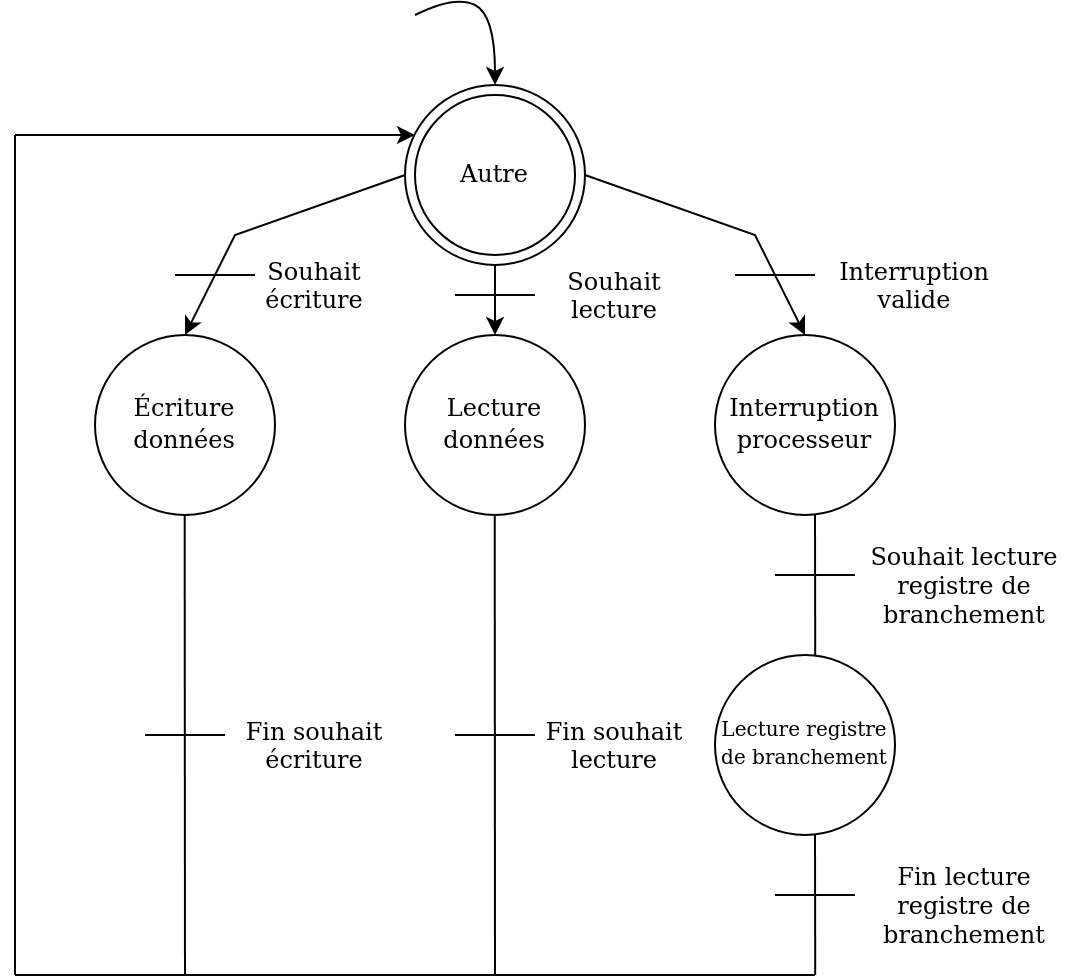
\includegraphics[width=0.8\linewidth]{figure/spec_automate_proc_ctrlmem.png}
	\caption{Comportement de l'ensemble processeur + contrôleur mémoire}
	\label{fig:spec_automate_proc_ctrlmem}
\end{figure} 

La figure ci-dessus représente le comportement de l'ensemble processeur + contrôleur mémoire.
Celui-ci possède trois cycles de fonctionnement.
Le processeur peut opérer des cycles de lecture et d'écriture dans les registres du contrôleur d'interruptions.
Le souhait d'écriture ou de lecture s'effectue par la mise à l'état bas du signal nCS\_IT.
La fin de ces cycles est notifiée par la mise à l'état haut du signal nAS.
Le terme "données" peut signifier la valeur des registres de configuration et également l'adresse de branchements.\\ 


\begin{figure}[H]
	\centering
	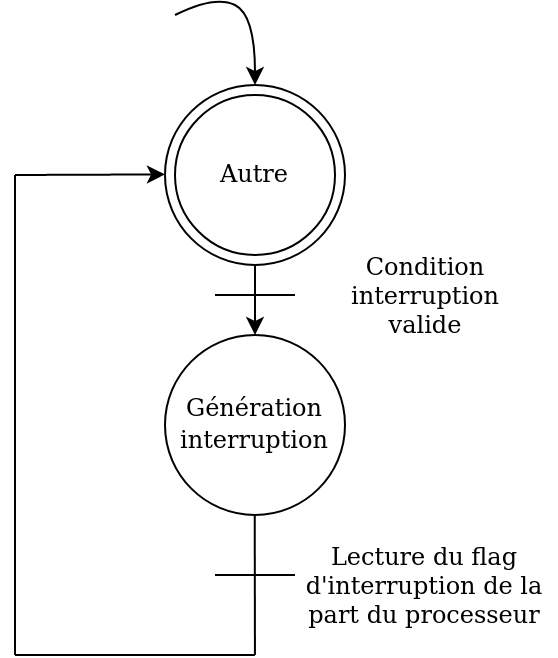
\includegraphics[width=0.5\linewidth]{figure/spec_automate_src_int.png}
	\caption{Comportement de l'entité source d'interruptions}
	\label{fig:spec_automate_src_it}
\end{figure} 

La figure ci-dessus est l'automate de l'entité source d'interruptions.
Lorsque la condition d'interruption est valide, le périphérique génère un signal en direction du contrôleur d'interruptions.
Ce signal reste actif jusqu'à la lecture du flag d'interruption de la part du processeur.

\subsection{Entrées et sorties du composant}

La caractérisation de l'environnement sous forme d'automates donne les relations d'entrées et sorties du circuit à concevoir avec les diverses entités.


\begin{figure}[H]
	\centering
	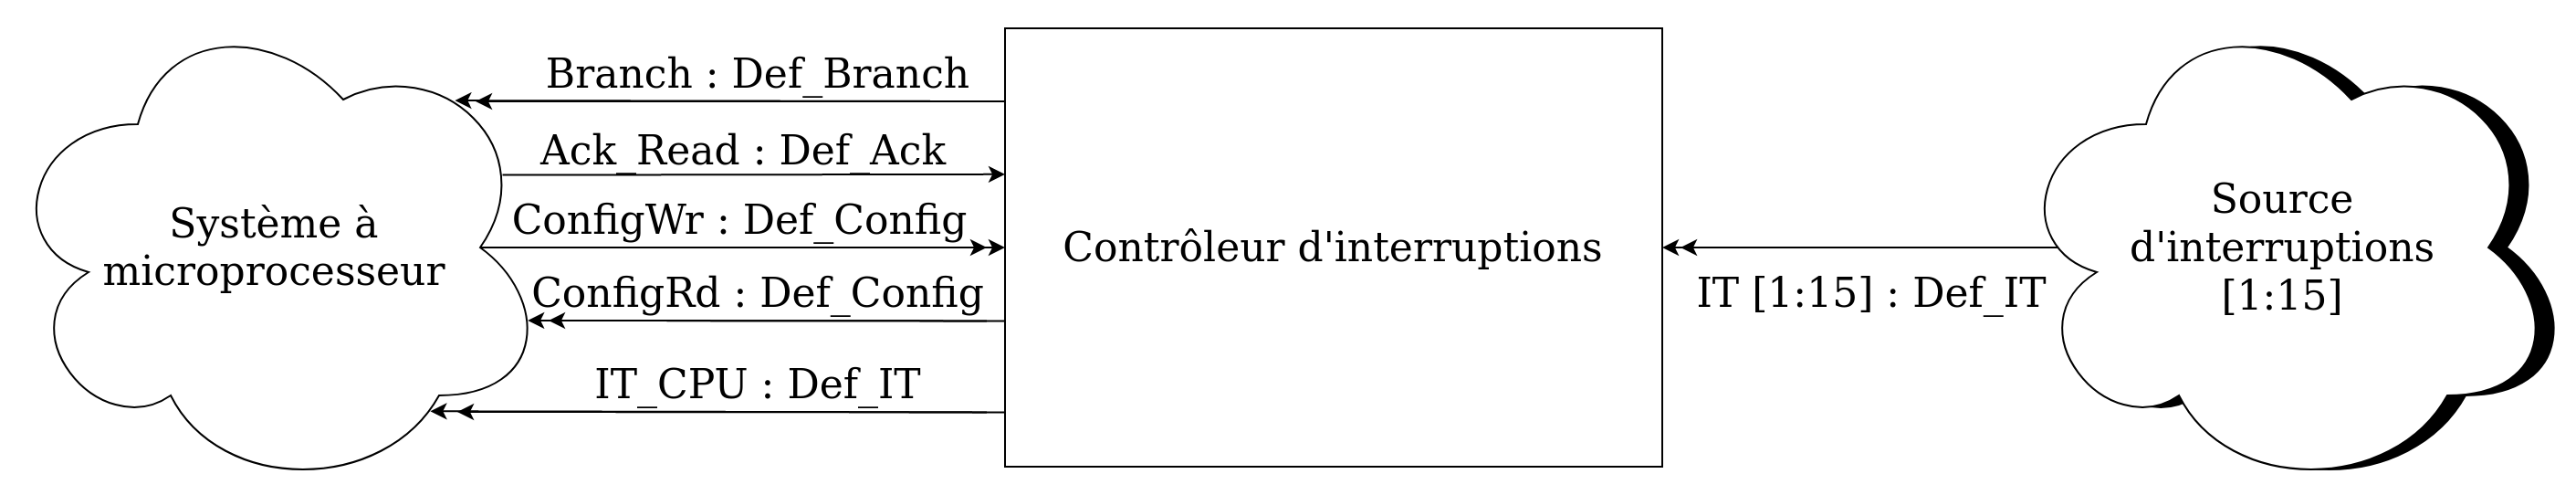
\includegraphics[width=1\linewidth]{figure/entrees_sorties_composant.png}
	\caption{Entrées et sorties du circuit à concevoir}
	\label{fig:entrees_sorties_composant}
\end{figure} 

\begin{table}[H]
	\centering
	\begin{tabular}{|c|c|c|c|c|}
		\hline
		Entités & Relation & Catégorie & Sens & Type\\
		\hline
		 & DataRd & Permanent & Sortie & Def\_Data \\
		Processeur + contrôleur mémoire & ConfigWr & Permanent & Entrée & Def\_Config \\
		& ConfigRd & Permanent & Sortie & Def\_Config \\
		& IT\_CPU & Permanent & Sortie & Def\_IT\\
		\hline
		Source d'interruptions [1:15] & IT [1:15] & Permanent & Entrée & Def\_IT\\
		\hline
	\end{tabular}
	\caption{Sens et rôle des signaux}
	\label{tab:entrees_sorties_composant}
\end{table}

\subsection{Spécifications fonctionnelles}
\subsection{Spécification des registres}
\subsection{Écriture des procédures de base pour l'emploi du circuit}
\subsection{Spécifications opératoires}
\subsection{Spécifications technologiques}